\documentclass[tikz,border=2pt]{standalone}
\usepackage{amsmath,amssymb}
\usepackage{tikz}

\begin{document}
% A tiny topological space: X = {a, b, c} with the open sets {}, {a}, {a,b}, X.
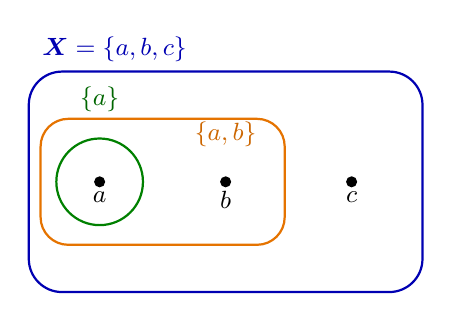
\begin{tikzpicture}[every node/.style={font=\small}]
	\draw[thick, blue!70!black, rounded corners=12pt] (-0.9,-0.9) rectangle (4.1,1.9);
	\node[blue!70!black, anchor=south west] at (-0.85,1.9) {$\boldsymbol{X}=\{a,b,c\}$};
	\draw[orange!90!black, thick, rounded corners=10pt] (-0.75,-0.3) rectangle (2.35,1.3);
	\draw[green!50!black, thick] (0,0.5) circle (0.55);
	\fill (0,0.5) circle (2pt) node[below] {$a$};
	\fill (1.6,0.5) circle (2pt) node[below] {$b$};
	\fill (3.2,0.5) circle (2pt) node[below] {$c$};
	\node[green!40!black, font=\small] at (0,1.55) {$\{a\}$};
	\node[orange!80!black, font=\small] at (1.6,1.1) {$\{a,b\}$};
\end{tikzpicture}
\end{document}
